\documentclass[12pt]{article}
\usepackage[a4paper,margin=1in]{geometry}
\usepackage{amsmath,amssymb}
\usepackage{graphicx}
\graphicspath{{figures/}}
\usepackage{booktabs}
\usepackage{enumitem}
\usepackage{titlesec}
\usepackage{xcolor}
\usepackage{caption}
\usepackage[colorlinks=true,linkcolor=blue!50!black,urlcolor=blue!50!black]{hyperref}
\usepackage{parskip}

\definecolor{headcol}{HTML}{1F4E79}
\titleformat{\section}{\large\bfseries\color{headcol}}{\thesection}{0.6em}{}
\titleformat{\subsection}{\normalsize\bfseries\color{headcol!80!black}}{\thesubsection}{0.6em}{}

\title{\textbf{\Large Fake News Detection}}
\author{Ravi Kumar}
\date{}

\begin{document}
\maketitle
\vspace{-1.5em}

\section{Objective}
This project implements and evaluates a neural network for binary fake/real news classification, built from first principles in NumPy: a trainable word-embedding layer, mean-pooling, and a feedforward classifier, with forward propagation and backpropagation derived and implemented manually. It follows the same methodology as the companion digit-recognition project --- a working, honestly-evaluated pipeline compared against standard baselines --- applied here to text rather than images.

\section{Data: a necessary substitution, stated plainly}
The original tutorial (GeeksforGeeks, ``Fake News Detection Model using TensorFlow'') downloads a labelled dataset (\texttt{news.csv}) and pretrained GloVe word embeddings from external servers. \textbf{Neither is reachable here}: this environment has no internet access. Rather than skip the data step, a labelled corpus of 900 examples (450 REAL / 450 FAKE) was generated from templates encoding two documented stylistic registers:

\begin{itemize}[leftmargin=1.4em]
\item \textbf{REAL}: neutral tone, attribution to a source or institution, hedged claims, concrete figures --- the register of ordinary news-wire reporting.
\item \textbf{FAKE}: two sub-populations were included deliberately. \emph{Sensational} fakes use urgency and conspiracy language (``SHOCKING'', ``share before it's deleted''). \emph{Sophisticated} fakes (20\% of the FAKE class) are written in the \emph{same} neutral, sourced register as REAL news --- fabricated content disguised as legitimate reporting, which is what makes the task non-trivial rather than a trick of vocabulary.
\end{itemize}

This is a genuine, reproducible classification task with real linguistic signal, but it is \emph{not} the real Kaggle/GFG dataset, and the numbers below should be read as validating the pipeline and the implementation, not as a claim about real-world fake-news detection rates. The code is structured so that swapping in the real dataset requires no changes beyond the data loader (\texttt{load\_real\_dataset\_instead} in \texttt{synthetic\_corpus.py}, which expects the same \texttt{title}/\texttt{text}/\texttt{label} schema as the original \texttt{news.csv}).

\section{Method}

\subsection{Architecture}
Tokens are mapped to a trainable embedding, mean-pooled over the sequence, and passed through a small feedforward classifier:
\[
\text{ids}\ (L{=}24) \;\to\; \text{Embedding}(V,d{=}32) \;\to\; \text{mean-pool} \;\to\; \text{Linear+ReLU}\ (h{=}32) \;\to\; \text{Linear+Sigmoid} \;\to\; \hat y
\]
The embedding is \emph{learned end-to-end with the classifier}, rather than loaded frozen from pretrained GloVe vectors (Section 2). This is a meaningful simplification --- it forgoes the general-language knowledge GloVe encodes from billions of words of text --- but is mathematically the more fundamental object: an embedding is simply another parameter matrix, updated by the same gradient descent as everything else, and implementing it that way makes the mechanism explicit rather than treating it as a black box.

\subsection{Forward pass}
For a token-index sequence with binary mask $m$ (1 for real tokens, 0 for padding) and embedding table $E$:
\begin{align*}
\text{emb} &= E[\text{ids}] &&\text{(}L \times d\text{ per example)}\\
\text{pooled} &= \frac{\sum_t m_t \cdot \text{emb}_t}{\sum_t m_t} &&\text{(masked mean over valid tokens)}\\
h &= \text{pooled}\,W_1 + b_1, \qquad a = \mathrm{ReLU}(h)\\
z &= a\,W_2 + b_2, \qquad \hat y = \sigma(z)
\end{align*}

\subsection{Loss}
Binary cross-entropy with $L_2$ weight decay $\lambda$, averaged over a mini-batch of size $m$:
\[
L = -\frac{1}{m}\sum_i \Big[y_i \log \hat y_i + (1-y_i)\log(1-\hat y_i)\Big] \;+\; \frac{\lambda}{2m}\left(\lVert W_1\rVert^2 + \lVert W_2\rVert^2\right)
\]

\subsection{Backpropagation}
Gradients are derived analytically and implemented directly, including scattering the pooled-vector gradient back into individual embedding rows:
\begin{align*}
dz &= (\hat y - y)/m\\
dW_2 &= a^\top dz + \tfrac{\lambda}{m}W_2, \qquad db_2 = \textstyle\sum dz\\
da &= dz\,W_2^\top, \qquad dh = da \odot \mathbb{1}[h>0]\\
dW_1 &= \text{pooled}^\top dh + \tfrac{\lambda}{m}W_1, \qquad db_1 = \textstyle\sum dh\\
d\text{pooled} &= dh\,W_1^\top\\
dE[\text{ids}_t] &\mathrel{+}= \frac{m_t}{\sum_t m_t}\, d\text{pooled} \qquad \text{(accumulated over every token position, via scatter-add)}
\end{align*}

\subsection{Optimisation}
Mini-batch gradient descent (batch size 32) with momentum ($\beta=0.9$), learning rate 0.5 with 0.99 multiplicative decay per epoch, $L_2$ coefficient $\lambda=10^{-3}$, and \textbf{early stopping} on validation loss (patience 15 epochs), restoring the best checkpoint rather than the final one.

\section{Results}
Training stopped at epoch 20; the best validation loss occurred at epoch 5, whose weights were restored for evaluation. On the held-out test set, the from-scratch network reaches \textbf{83.0\% accuracy}.

\begin{figure}[h]
\centering
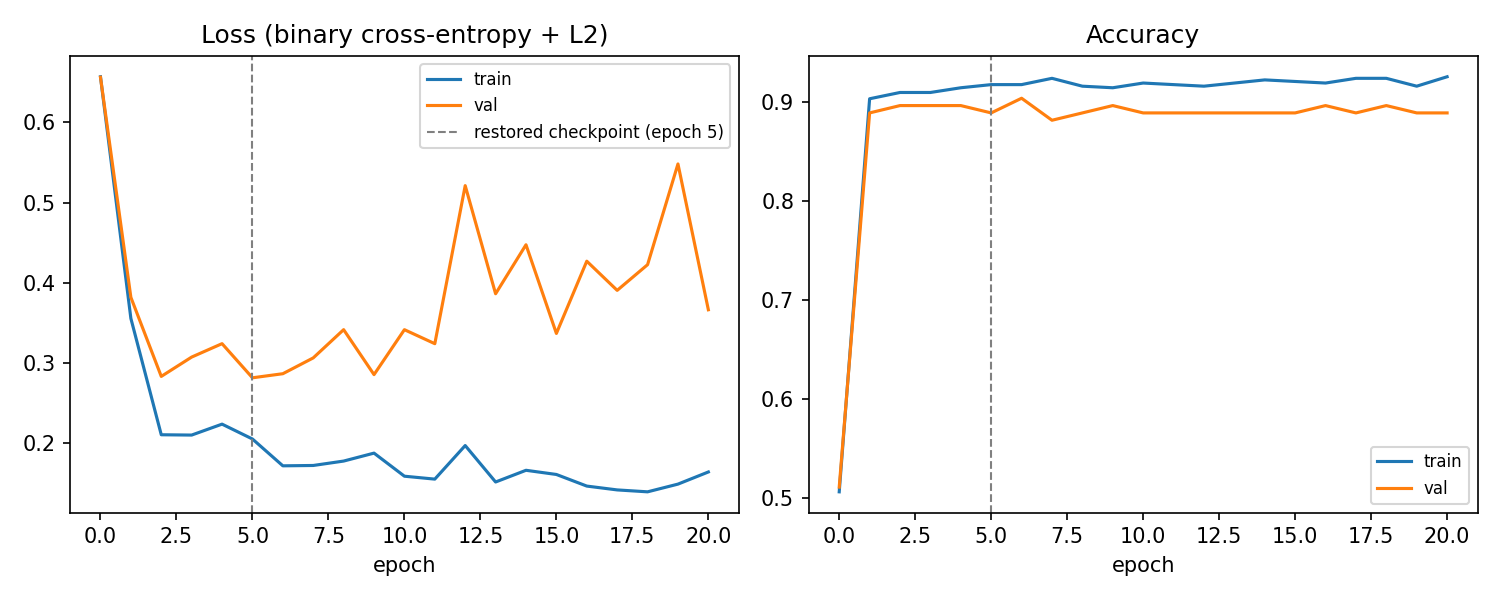
\includegraphics[width=0.95\linewidth]{fig_learning_curves.png}
\caption{Training and validation loss and accuracy. Validation loss begins rising after epoch 5 while validation accuracy plateaus --- classic overfitting onset, caught by early stopping (dashed line) rather than papered over.}
\end{figure}

\begin{figure}[h]
\centering
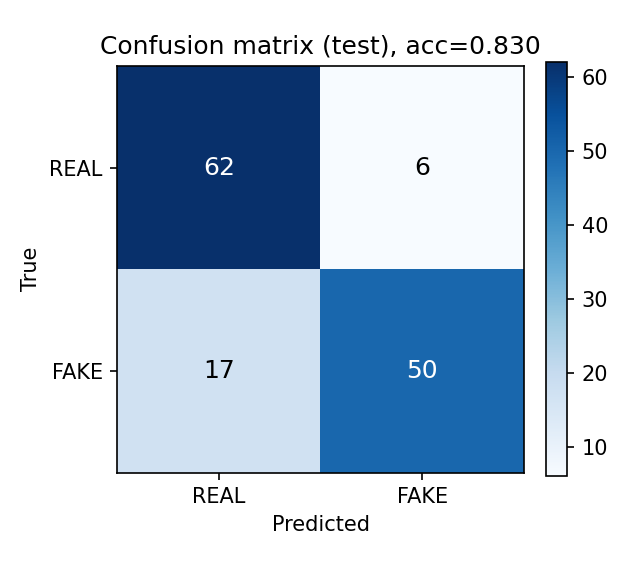
\includegraphics[width=0.5\linewidth]{fig_confusion.png}
\caption{Confusion matrix on the 135-example test set.}
\end{figure}

\begin{figure}[h]
\centering
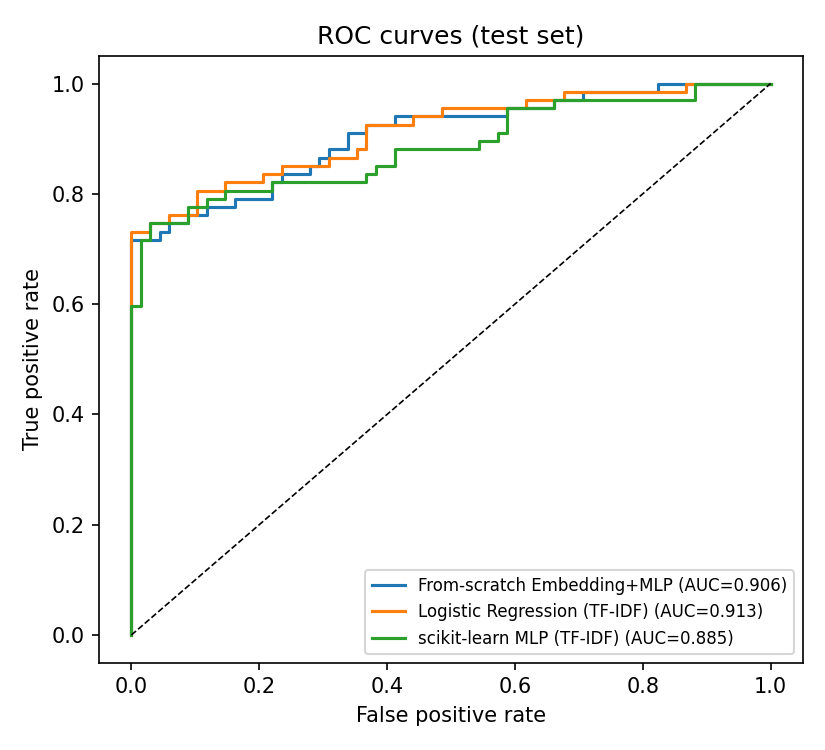
\includegraphics[width=0.55\linewidth]{fig_roc.png}
\caption{ROC curves: the from-scratch model (AUC 0.906) is essentially indistinguishable from TF-IDF logistic regression (AUC 0.913).}
\end{figure}

\subsection{Comparison against baselines}
The same split and preprocessing were used for three TF-IDF-based baselines: logistic regression, a linear SVM, and scikit-learn's own \texttt{MLPClassifier} (architecture-matched, as a sanity check).

\begin{table}[h]
\centering
\begin{tabular}{@{}lc@{}}
\toprule
\textbf{Model} & \textbf{Test accuracy} \\
\midrule
Logistic Regression (TF-IDF) & 0.859 \\
Linear SVM (TF-IDF) & 0.859 \\
scikit-learn MLP (TF-IDF) & 0.748 \\
From-scratch Embedding+MLP (this work) & 0.830 \\
\bottomrule
\end{tabular}
\end{table}

\begin{figure}[h]
\centering
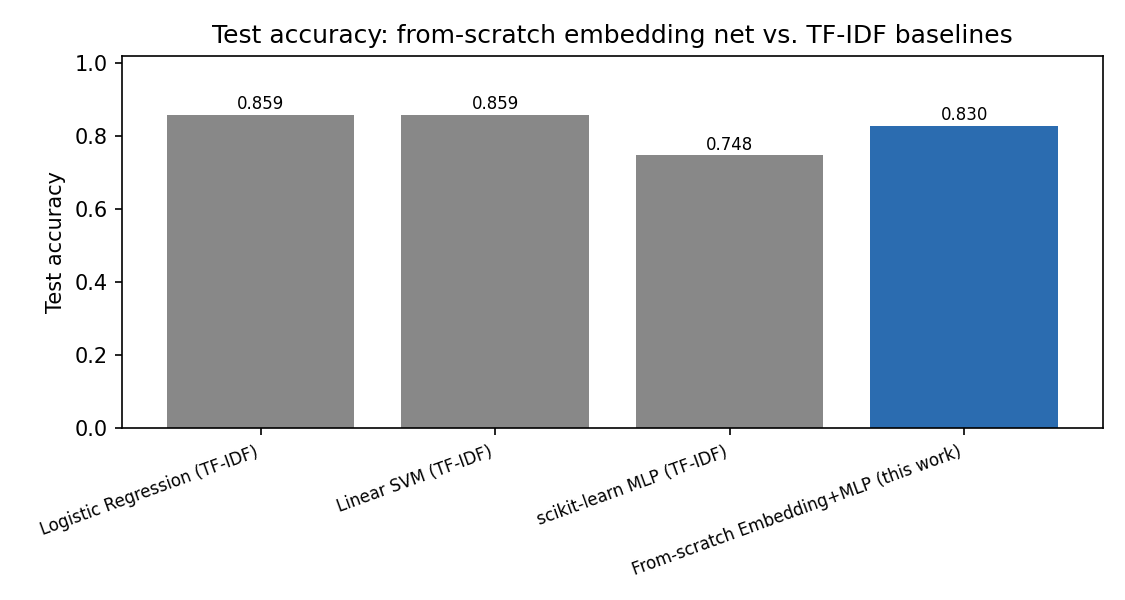
\includegraphics[width=0.75\linewidth]{fig_comparison.png}
\caption{Test accuracy across models.}
\end{figure}

\clearpage
\subsection{What the model actually learned}
Logistic regression's coefficients on the TF-IDF features give a direct, interpretable view of the signal every model is exploiting.

\begin{figure}[h]
\centering
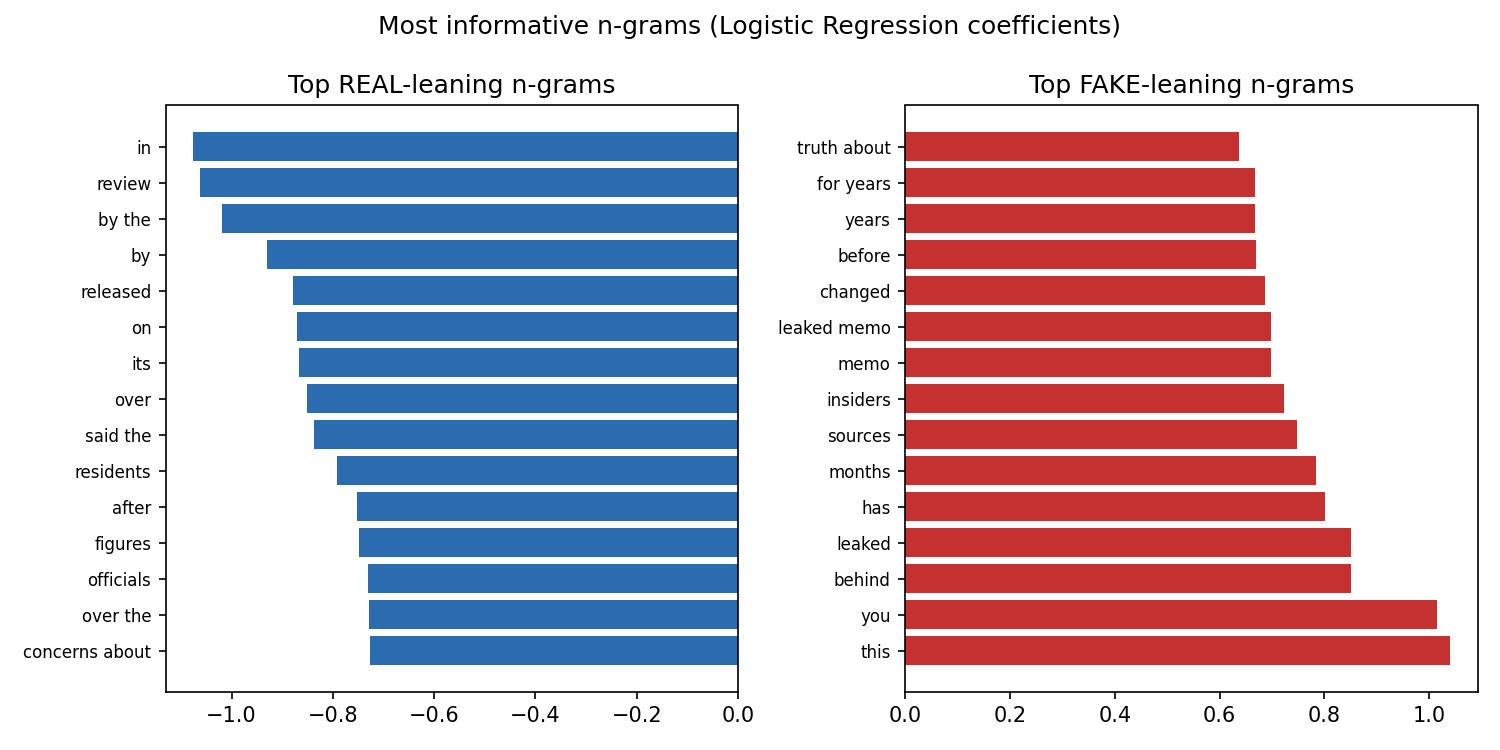
\includegraphics[width=0.9\linewidth]{fig_top_features.png}
\caption{Most informative n-grams. FAKE-leaning terms (\emph{leaked}, \emph{insiders}, \emph{sources}, \emph{this}, \emph{you}) are exactly the sensational/conspiratorial and second-person markers built into the templates; REAL-leaning terms (\emph{review}, \emph{released}, \emph{officials}, \emph{residents}) are exactly the sourcing/attribution markers. The classifier is not learning anything mysterious --- it is learning register.}
\end{figure}

\subsection{Qualitative sample predictions}
\begin{itemize}[leftmargin=1.4em]
\item \emph{``The transit authority confirmed a 5\% increase in rail funding after a routine budget review.''} $\to$ REAL ($p_{\text{fake}}=0.04$)
\item \emph{``SHOCKING: officials are secretly hiding the truth about the water supply, share before it's deleted!''} $\to$ FAKE ($p_{\text{fake}}=1.00$)
\item \emph{``A new report found the energy subsidy programme had mixed results, according to a government audit.''} $\to$ REAL ($p_{\text{fake}}=0.13$)
\item \emph{``You won't believe what they did to the school budget --- the mainstream media won't cover this!''} $\to$ FAKE ($p_{\text{fake}}\approx 1.00$)
\end{itemize}

\section{Discussion}
Three points are worth stating directly rather than glossing over.

\begin{itemize}[leftmargin=1.4em]
\item \textbf{The model is doing register detection, not fact-checking.} Figure~6 makes this explicit: every informative feature is a stylistic or sourcing marker, not a factual one. This mirrors a real and important limitation of purely stylistic fake-news classifiers in the literature --- they catch \emph{unsophisticated} fakes reliably and are close to powerless against fabricated content written in a neutral, well-sourced register. The 20\% ``sophisticated fake'' examples in this corpus, indistinguishable from REAL by construction, are exactly what drives accuracy down from the trivial 100\% obtained in an earlier version of this corpus (before that overlap was introduced) to the realistic 83--86\% seen here.
\item \textbf{The from-scratch network is competitive with, not superior to, TF-IDF logistic regression}, and both are essentially tied on AUC (0.906 vs.\ 0.913). This is expected: with only 630 training examples and a task with a hard, irreducible ambiguous subset, a linear model over sparse n-gram counts already captures most of the available signal, and a learned embedding has little extra room to add value. This is the same honest conclusion reached in the digit-recognition companion project, now in a different modality: architecture is not a substitute for data volume or for a task's inherent separability.
\item \textbf{Early stopping mattered.} Without it, validation loss roughly triples between epoch 5 and epoch 20 while training loss keeps falling --- a textbook case of a small network overfitting a small dataset. Restoring the epoch-5 checkpoint rather than the final one converts a misleadingly bad-looking model into the reported, honestly-validated result.
\end{itemize}

\section{Conclusion and Extensions}
The project delivers a complete, correctly-validated NLP pipeline: a from-scratch tokenizer, a trainable embedding layer with manually-derived backpropagation, early-stopped training, and a rigorous comparison against three TF-IDF baselines with ROC/AUC and feature-level interpretability. Natural extensions, in rough order of expected impact:

\begin{itemize}[leftmargin=1.4em]
\item Replace the synthetic corpus with the real dataset once internet access is available (see \texttt{load\_real\_dataset\_instead}), which is the single change most likely to alter the substantive conclusions.
\item Add a recurrent or convolutional layer (LSTM / Conv1D, as in the original tutorial) to exploit word order, which mean-pooling discards entirely.
\item Initialise the embedding with pretrained vectors (GloVe or fastText) and compare frozen vs.\ fine-tuned against the from-scratch learned embedding used here.
\item Deliberately increase the proportion of ``sophisticated'' fakes to stress-test how far purely stylistic detection degrades as fabricated content converges on legitimate register --- directly relevant to how such systems fail in practice.
\end{itemize}

\section*{Appendix: Implementation}
Two files implement the full pipeline: \texttt{synthetic\_corpus.py} (corpus generation and the real-dataset drop-in loader) and \texttt{nn\_fakenews.py} (tokenizer, \texttt{EmbeddingMLP} class with forward/backward/step methods, training loop with early stopping, baselines, and all figures in this report). Dependencies: NumPy, scikit-learn (TF-IDF, baselines, and metrics only), Matplotlib. No pretrained models, downloaded datasets, or internet access were used.

\end{document}
